\textbf{Цель работы:} \\\indent
1) измерение объемов форвакуумной и высоковакуумной частей установки;\\\indent 
2) определение скорости откачки системы в стационарном режиме, а также 
по ухудшению и по улучшению вакуума. \\\indent
\textbf{Оборудование:} вакуумная установка с манометрами: масляным, 
термопарным и ионизационным. \\ 
\section*{Экспериментальная установка}

Установка состоит из форвакуумного баллона (ФБ), высоковакуумного диффузионного
насоса (ВН), высоковакуумного баллона (ВБ), масляного (М) и ионизационного (И) манометров,
термопарных манометров ($M_1$ и $M_2$), форвакуумного насоса (ФН) и кранов 
($K_1, \dots, K_6$).

\begin{figure}[h!]
    \centering
    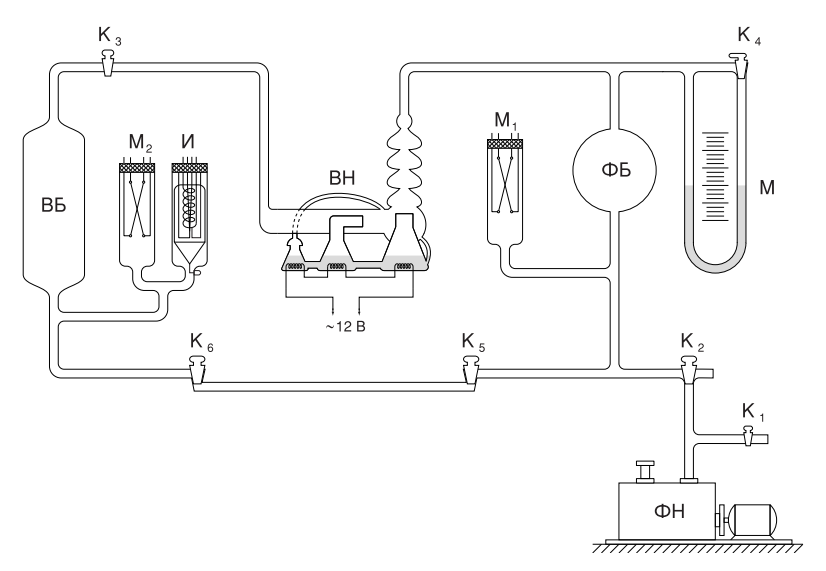
\includegraphics[height=8cm]{setup.png}
    \caption{Схема экспериментальной установки}
\end{figure}

\newpage

% \subsection*{Форвакуумный насос}
% \subsection*{Диффузионный насос}
% Действие этого насоса основано на диффузии молекул разряженного воздуха
% в струю паров масла. Молекулы газа увлекаются струей и не возвращаются назад. 
% На из место попадают новые и так далее... Таким образом, степень разряженности
% газа в окрестности струи увеличивается. 
% \begin{wrapfigure}{i}
%     \centering
%     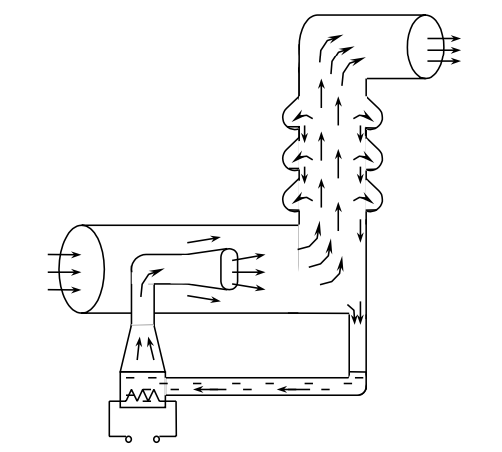
\includegraphics[height=6cm]{oildefusepump.png}
%     \caption{Схема работы диффузионного насоса}
% \end{wrapfigure}
%
% \subsection*{Термопарный манометр}
%

\section*{Теоретические сведения}
\subsection*{Откачка}
Пусть $W$ - объем газа, удаляемого из сосуда при данном давлении за 
единицу времени; $Q_{\text{д}}$ - кол-во газа, деосбирующегося с поверхности 
откачиваемого объема в ед.вр.; $Q_{\text{и}}$ - количество газа, принятое
извне; $Q_{\text{н}}$ - поток газа, поступающего из насоса назад в
откачиваемую систему. 
\begin{align}
    d(VP) &= (Q_{\text{д}} + Q_{\text{и}} + Q_{\text{н}}) dt \label{eq:dif}\\
    -VdP &= (PW - Q_{\text{д}} - Q_{\text{и}} - Q_{\text{н}}) dt
\end{align}
При достижении предельного вакуума $P_{\text{пр}}$:
\begin{align}
    \frac{dP}{dt} &= 0\\ 
    P_{\text{пр}}W = Q_{\text{д}} + Q_{\text{и}} + Q_{\text{н}} \Rightarrow W &= \frac{\sum Q_{\text{i}}}{P_{\text{пр}}}
\end{align}
Из \ref{eq:dif} и считая $Q_{\text{д}}, Q_{\text{и}}, Q_{\text{н}}$
постоянными, получаем:
\begin{equation}
P - P_{\text{пр}} = (P_0 - P_{\text{пр}})\exp{\left (-\frac{W}{V}t\right )}
\end{equation}
где $P_0$ - начальное давление ($P_0 \gg P_{\text{пр}}$) $\Rightarrow$
\begin{equation}
    P = P_0\exp(-\frac{W}{V}t)
\end{equation}

\subsection*{Течение газа через трубку}
Характер течения газа определяется размерами системы и длиной свободного 
пробега молекул. При понижении давления до форвакуумного длина свободного 
пробега меньше диаметра трубы, поэтому течение определяется вязкостью воздуха. 
При высоком вакууме роль длины свободного пробега молукл принимет диаметр
трубки. \\\indent 
Для количества газа, протекающего через трубку при высоком вакууме:
\begin{equation}
    \frac{d(PV)}{dt} = \frac{4}{3}r^3 \sqrt{\frac{2\pi RT}{\mu}} \frac{P_2 - P_1}{L}
\end{equation}
Тогда пропускная способность трубы ($P = P_2, P_1 \ll P_2$):
\begin{equation}
    C_{\text{тр}} = \left (\frac{dV}{dt} \right ) = \frac{4}{3}\frac{r^3}{L} \sqrt{\frac{2\pi RT}{\mu}}  
\end{equation}




